Following the
literature~\cite{Ghiya96,Sagiv96,marron06static},
we define the shape attribute for a pointer $\p$
as:
\begin{eqnarray*}
  \p.\shape = \left\{ \begin{array}{@{}rl@{}}
    \Cycle & \mbox{If a cycle can be reached from $\p$} \\ 
    \Dag & \mbox{Else if a DAG can be reached from $\p$} \\
    \Tree & \mbox{Otherwise} \\
  \end{array} \right.
\end{eqnarray*}
where the heap is visualized as a directed graph, and cycle
and DAG have there natural graph-theoretic meanings. For each
pointer variable, our analysis computes the shape attribute
of the data structure pointed to by the variable.  We use the
code fragment in Fig.~\ref{fig:motiv1} to motivate the need
for a field sensitive shape analysis.

\begin{figure}[t]
\begin{center}
  \scalebox{.99}{
    \begin{tabular}{c}
      {\small \tt
        \begin{tabular}[b]{rl}
          &int main() \{ \\
	  {\em \scriptsize S1:}& \quad tree root; \\
	  {\em \scriptsize S2:}& \quad \ldots        \\
          {\em \scriptsize S3:}& \quad mirror(root); \\
          {\em \scriptsize S4:}& \quad treeAdd(root); \\ 
          {\em \scriptsize S5:}& \quad \ldots \\ 
          &\} \\ \\
          & void mirror(tree t) \{ \\
          {\em \scriptsize S11:}& \quad tl  = t->left; \\
          {\em \scriptsize S12:}& \quad tr = t->right; \\
          {\em \scriptsize S13:}& \quad mirror(tl); \\
          {\em \scriptsize S14:}& \quad mirror(tr); \\
          {\em \scriptsize S15:}& \quad t->left  = tr; \\
          {\em \scriptsize S16:}& \quad t->right = tl; \\
          &\} \\ \\
	  & int treeAdd(tree t) \{     \\ 
	  {\em \scriptsize S21:}& \quad if (t == NULL)           \\ 
	  {\em \scriptsize S22:}& \quad \quad return 0;           \\ 
	  {\em \scriptsize S23:}& \quad tl = t$\rightarrow$left;    \\
          {\em \scriptsize S24:}& \quad treeAdd(tl); \\
          {\em \scriptsize S25:}& \quad tr = t$\rightarrow$right; \\
	  {\em \scriptsize S26:}& \quad treeAdd(tl); \\
	  {\em \scriptsize S27:}& \quad t$\rightarrow${num} = tl$\rightarrow${num} + tr$\rightarrow${num}; \\
	  &\}
        \end{tabular}
      } \\ \scalebox{0.80}{(a)} \\ \\ %\hline \\ \\
      {\small \tt
        \begin{tabular}[b]{l}
          typedef struct treenode tree;\\
          struct treenode \{ \\
            \quad int num; \\
            \quad tree *left; \\
            \quad tree *right; \\
            \};
        \end{tabular}
      } 
      \hskip -10mm\includegraphics[scale=
        .4]{Figures/tree_grph.eps} \\
      \scalebox{0.8}{(b)} \\ %\hline
    \end{tabular}}
\end{center}
\caption{\label{fig:motiv1} A motivating example. The program
  (a) manipulates  the heap structures created by using the
  basic data structure as shown in (b).}
\end{figure}


\begin{figure}[t]
\begin{center}
  {\small \tt 
    \begin{tabular}[b]{|l|@{}c@{}|} \hline
      {\rm Stmt} & {\rm Path matrix  $P_F$ after the stmt}  \\ \hline
      \multicolumn{2}{c}{} \\ \hline
      {\em \scriptsize S1} &
      \begin{tabular}{|p{3mm}||p{6mm}|p{12mm}|p{22mm}|} \hline
        &  t         & tl        & tr   \\ \hline\hline
  	t  	& $\emptyset$   & ${\tt \{\fieldD{\lft}{}\}}$    & $\emptyset$ \\ \hline
  	tl  & $\emptyset$   & $\emptyset$   & $\emptyset$   \\ \hline
  	tr  & $\emptyset$   & $\emptyset$   & $\emptyset$   \\ \hline
      \end{tabular} \\ \hline
      \multicolumn{2}{c}{} \\ \hline
      {\em \scriptsize S2} &				
      \begin{tabular}{|p{3mm}||p{6mm}|p{12mm}|p{22mm}|} \hline
        &  t         & tl        & tr   \\ \hline\hline
  	t  	& $\emptyset$   & ${\tt \{\fieldD{\lft}{}\}}$    & ${\tt \{\fieldD{\rht}{}\}}$ \\ \hline
  	tl  & $\emptyset$   & $\emptyset$   & $\emptyset$   \\ \hline
  	tr  & $\emptyset$   & $\emptyset$   & $\emptyset$   \\ \hline
      \end{tabular} \\ \hline
      \multicolumn{2}{c}{} \\ \hline
      {\em \scriptsize S5} &				
      \begin{tabular}{|p{3mm}||p{6mm}|p{12mm}|p{22mm}|} \hline
        &  t         & tl        & tr   \\ \hline\hline
  	t  	& $\emptyset$   & $\emptyset$    & ${\tt \{\fieldD{\rht}{},\fieldD{\lft}{} \}}$ \\ \hline
  	tl  & $\emptyset$   & $\emptyset$   & $\emptyset$   \\ \hline
  	tr  & $\emptyset$   & $\emptyset$   & $\emptyset$   \\ \hline
      \end{tabular} \\ \hline
      \multicolumn{2}{c}{} \\ \hline
      {\em \scriptsize S6} &				
      \begin{tabular}{|p{3mm}||p{6mm}|p{12mm}|p{22mm}|} \hline
        &  t         & tl        & tr   \\ \hline\hline
  	t  	& $\emptyset$   & ${\tt \{\fieldD{\rht}{}\}}$   & ${\tt \{\fieldD{\lft}{} \}}$ \\ \hline
  	tl  & $\emptyset$   & $\emptyset$   & $\emptyset$   \\ \hline
  	tr  & $\emptyset$   & $\emptyset$   & $\emptyset$   \\ \hline
      \end{tabular} \\ \hline
    \end{tabular}				
  }
\end{center}
\caption{\label{fig:motiv2}  Paths computed  by  our analysis
  for  the  program  in  Figure~\ref{fig:motiv1}(a)  as  path
  matrix $P_F$.   The entry $P_F[x,y]$  lists  the  paths   between  pointer
  variables $x$ and $y$.}
\end{figure}

\begin{example}{\rm
    The program in Fig.~\ref{fig:motiv1}(a) creates a binary
    tree rooted at {\tt root} (not shown) and uses the
    function {\tt mirror} to create its mirror image {\em
      in-situ}. The program then calls {\tt treeAdd} on the
    mirrored tree to perform the additions of its left and
    right subtrees recursively. 
    
    If it can be inferred that the shape of the argument to
    the function {\tt treeAdd} is indeed \Tree, then a
    parallelizing compiler can schedule the two recursive
    calls to {\tt treeAdd} on lines {\em S24} and {\em S26}
    in parallel. This is possible because these two calls 
    do not access any common region of heap, and hence they
    can proceed independently. 
    
    The inference of the shape of the argument of the {\tt
      treeAdd} depends on the execution of {\tt
      mirror}. Even when called with an argument that has a
    shape of \Tree, the function {\tt mirror} temporarily
    changes the shape to a \Dag\ (due to assignments on line
    {\em S12} and {\em S15}, both {\tt t$\rightarrow$left}
    and {\tt t$\rightarrow$right} point to the same node {\tt
      tr}). The shape is reverted back to \Tree\ at line {\em
      S26}. 
 
    Field   insensitive   shape   analysis   algorithms   use
    conservative  kill  information and  hence  they are,  in
    general,  unable  to  infer  the  shape  transition  from
    \Cycle\ to  \Dag\ or from  \Dag\ to \Tree.   For example,
    the   algorithm  by   Ghiya   et.~al.~\cite{Ghiya96}  can
    correctly  report  the  shape  transition from  \Tree\  to
    \Dag\  (at  {\em  S15})  but  fails to  infer  the  shape
    transition  from  \Dag\ to  \Tree\ (at  {\em S16}).   Our
    analysis, on  the other hand,  keeps track of  the fields
    involved  in creation  of the  DAG at  {\em  S15} ({\tt
      t$\rightarrow$left} and {\tt t$\rightarrow$right}), and
    therefore it is able to  restore the shape to Tree when
    {\tt        t$\rightarrow$right}        is        updated.
    \hfill\psframebox{}}
\end{example}

We now show how we have incorporated limited field sensitivity
at each program point in our shape analysis. The details of our
analysis will be presented later (Sect.\ref{sec:Analysis}).

\begin{example}{\rm 
The  statement at  {\em S15}  creates a  new DAG structure
reachable  from {\tt t},  because there  are two  paths ({\tt
  t$\rightarrow$\lft} and  {\tt t$\rightarrow$\rht}) reaching
{\tt tr}.   A field  sensitive shape analysis  algorithm must
remember all  paths from {\tt  t} to {\tt tr}.   Our analysis
approximates  a path  between  two pointer  variables by  the
first  field that is  dereferenced on  the path.  Further, as
there  may  be  an  unbounded  number of  paths  between  two
variables, we  use $k$-limiting~\cite{Jones79} to approximate
the number of paths starting at a given field.

Our  analysis  remembers   the  path  information  using  the
following:  (a)  $P_F$: Path  matrix  that  stores the  first
fields  of the  paths between  two pointers  and  (c) Boolean
Variables  that remember the  fields directly  connecting two
pointer   variables.  Figures~\ref{fig:motiv2} shows  the
values computed  for $P_F$ and boolean variables by our
analysis for the  example program in Figure~\ref{fig:motiv1}(a). In
this case,  the fact that the  shape of the  variable {\tt t}
becomes \Dag\ after {\em S15}  is captured by  the following
boolean functions\footnote{The functions  and values shown in
  this example and in Fig.~\ref{fig:motiv2} are simplified
  to avoid references to concepts not defined yet.}  :
\begin{eqnarray*} 
  \mtt{t}_{\subD} &=& ({\lft}_{\mtt{t}\ \mtt{tr}} \wedge (\num{\DFM{\mtt{t}}{\mtt{tr}}} > 1)), \\ 
  \qquad {\lft}_{\mtt{t}\ \mtt{tr}} &=& \true. 
\end{eqnarray*}
Where ${\lft}_{\mtt{t}\ \mtt{tr}}$ is a boolean variable that
is \true\ because  the \lft\ field of \mtt{t} points to \mtt{tr}, 
$P_F$  is field sensitive  Path matrix, $\num{P_F[\mtt{t},\mtt{tr}]}$ 
  is the  count of number of paths between \mtt{t} and \mtt{tr}.

The  functions simply  say that  variable \mtt{t}  reaches a
DAG because  there are more than  one paths ($\num{P_F[\mtt
      {t},\mtt{tr}]} >  1$) from \mtt{t} to \mtt{tr}. It also
keeps  track  of the  path  ${\lft}_{\mtt{t}\  \mtt{tr}}$ that  is
involved in  the creation of  the DAG.  Later,  at statement
{\em S16}, the path due \mtt{t}$\rightarrow$\rht\ between \mtt{t} 
and  \mtt{tr} is broken,  causing $\num{P_F[\mtt{t},\mtt{
      tr}]} =  1$.  This  causes $\mtt{t}_{\subD}$  to become
\false.  Note  that  we  {\em  do not}  evaluate  the  boolean
functions   immediately,   but   associate  the   unevaluated
functions with the  statements. When we want to  find out the
shape  at  a  given  statement,  only then  we  evaluate  the
function  using  the  values   from  $P_F$  and  the  boolean
variables at that statement.
\hfill\psframebox{}}
\end{example}

We  now formalize  the  intuitions presented  in the  example
above, starting  with the concepts necessary  to describe our
field sensitive shape analysis technique.
